\chapter{Reconstructing  CT Signals}

In the previous lecture we focused on sampling of CT signals to produce a DT signal $x[n] = x(nT)$ with sample index $n$ and sample time $T$. In this lecture we consider \emph{reconstruction}, converting from a DT signal $x[n]$ to a CT signal $x(t)$ using a sample time $T$ as the spacing between samples. Ideally a conversion from $x(t)$ to $x[n]$ and back again would result in identical signal. 

\section{Reconstruction Theory}
Given a DT signal $x[n]$ and a sample spacing $T$, we can define a corresponding CT signal as 
\[
x_p(t) = \sum\limits_{n = -\infty}^{\infty} x[n] \, \delta(t-nT)
\]
the impulse train with each impulse weighted by the DT signal.

CT signal reconstruction can be viewed from two different (but equivalent) perspectives. In the time domain perspective, the CT signal $x(t)$ corresponding to a DT signal $x[n]$ can be viewed as \emph{interpolation}, where the values of the CT signal are equal to the DT signal at intervals of the sample time, i.e. $x(nT) = x[n]$, and in between the value of $x(t)$ is interpolated. If the interpolation is of zero-order, the value at $x(nT)$ is held constant until $x(nT+T)$. This is called a \emph{zero-order hold}, and can mathematically modeled as convolution of the weighted impulse train with a pulse $p(t) = u(t) - u(t-T)$ whose width is the sample time, called the interpolation function.
\[
y(t) = p(t)*x_p(t)
\]
This is illustrated below
\begin{center}
  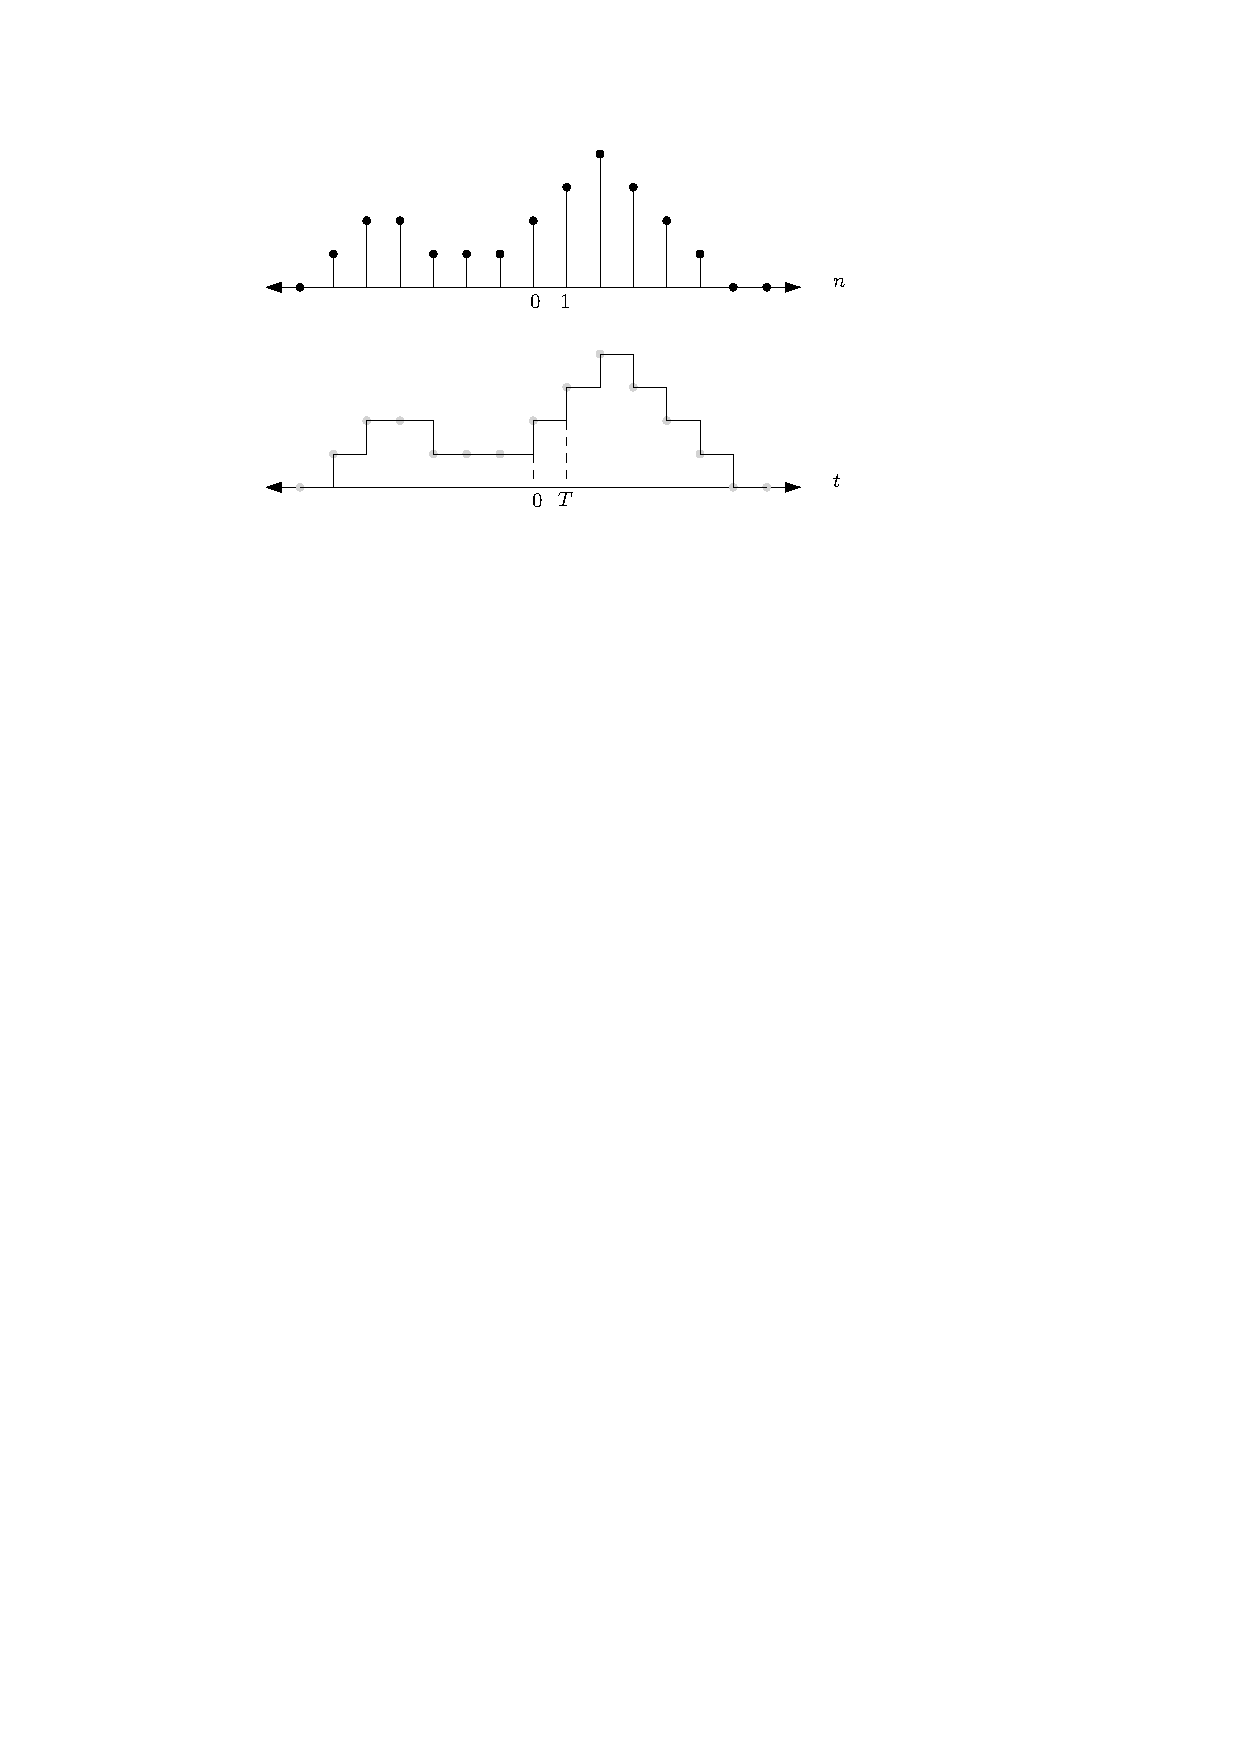
\includegraphics[scale=1]{graphics/zero-order-hold-interp.pdf}
\end{center}

The zero-order hold is not a very accurate representation of a band-limited signal. So, what interpolation function is optimal?

To answer this question we can turn to the alternative perspective on reconstruction, that of the frequency domain. Recall the sampled signal $x(nT)$ in the frequency domain can be viewed as the summation of the Fourier transform of $x(t)$, $X(j\omega)$, and periodic replicas or images centered at multiples of the sampling frequency. If we assume the original signal was band-limited and sampled appropriately (using the Nyquist criteria), then if we ideal low-pass filter the sampled signal we will preserve the central portion of the Fourier spectrum that corresponds to the original signal, and chop off the images. For this reason the reconstruction filter is also called an anti-imaging filter.

\begin{center}
  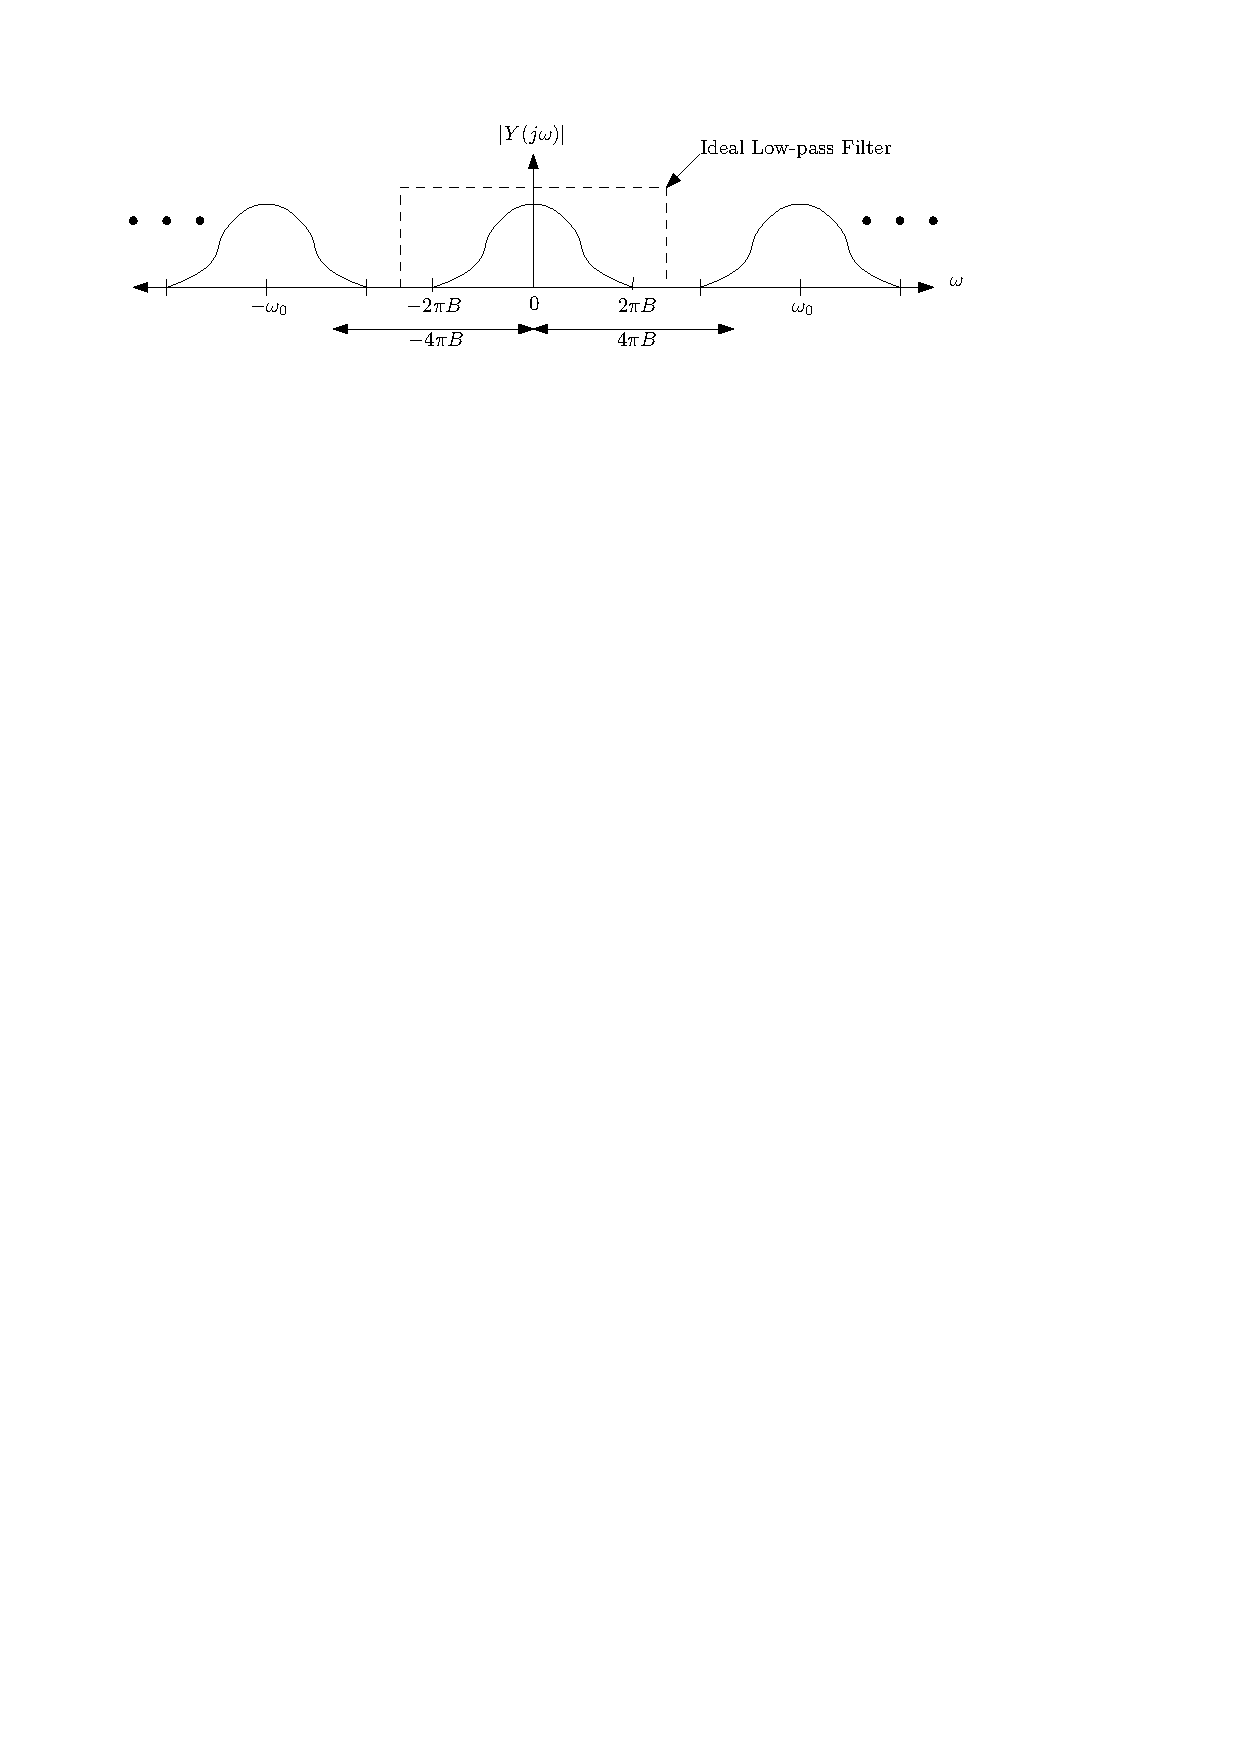
\includegraphics[scale=1]{graphics/bandlimitedreconstructed1.pdf}
\end{center}

Recall filtering is multiplication the frequency domain and convolution in the time domain, so the optimal interpolation function corresponds to the impulse response of the ideal low-pass filter with cutoff frequency $\omega_c = 2\pi B$, a sinc function.

\[
h(t) = \mathcal{F}^{-1} \left\{ H(j\omega) \right\} = \frac{1}{2\pi} \int\limits_{\-\omega_c}^{\omega_c} e^{j\omega t} \; d\omega = \frac{1}{\pi t}\sin(\omega_c t) 
\]

Thus the ideal ideal interpolation function is the sinc function, and reconstruction is low-pass filtering of the weighted impulse train $x_p(t)$ \footnote{As an aside this also gives an intuitive view of convolution with an impulse train, as interpolation}.

\section{Practical Reconstruction}

As we have seen before we cannot physically represent the impulse train nor the ideal low-pass filter. Thus practical reconstruction uses an approximation of the ideal reconstruction filter by a digital-to-analog converter (DAC), followed by a causal (and thus physically possible) low-pass filter.

\subsection{Zero-order hold using an R-2R ladder}

A zero-order hold DAC can be implemented by a circuit called a resistor ladder. Consider a digital output with $N$ bits and a reference voltage $V_{ref}$ (for example an 8-bit output port on a micro-controller using CMOS 3.3v logic).

If this port is connected to a resistor network consisting of resistor values $R$ and $2R$ as follows

\begin{center}
  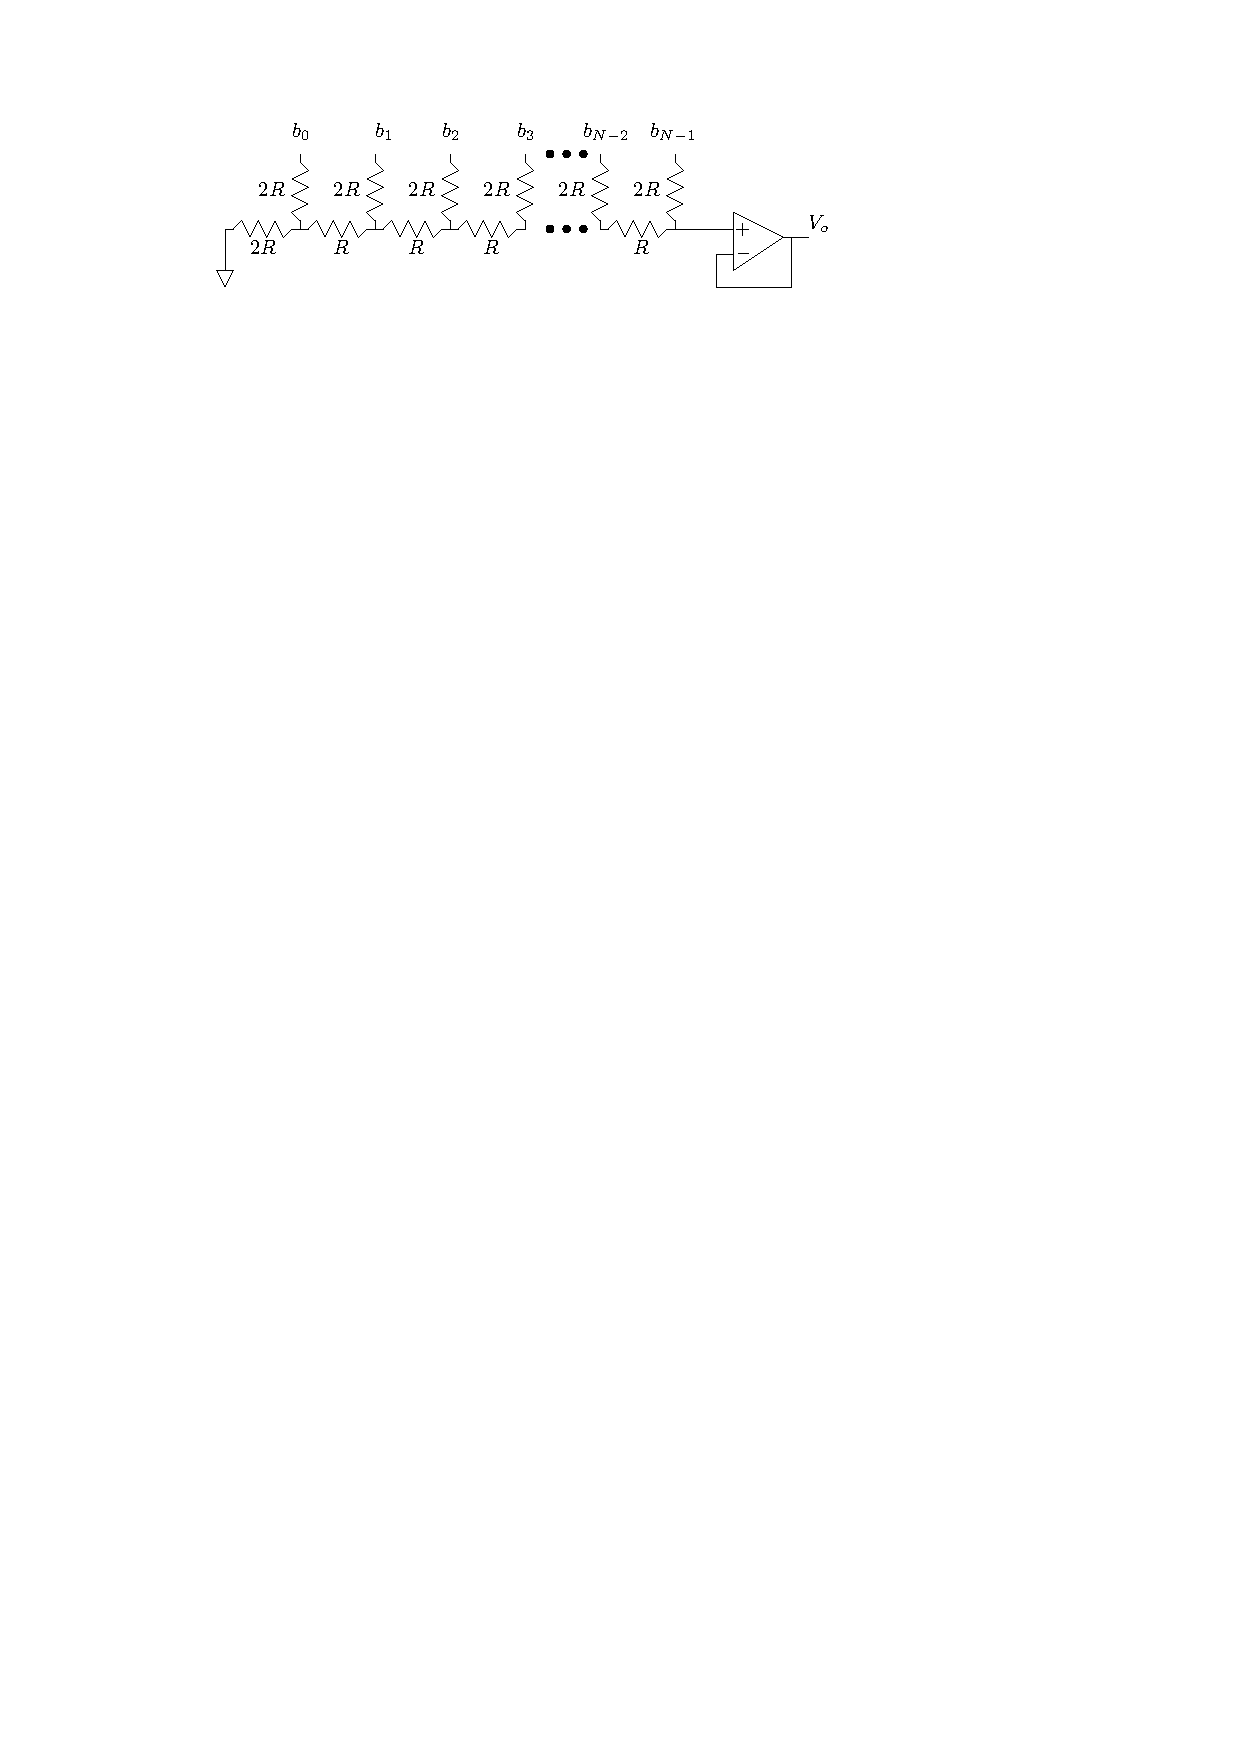
\includegraphics[scale=1]{graphics/resistor-ladder.pdf}
\end{center}


then depending on the bit pattern at the output port $V$, the output of the buffer op-amp will be
\[
V_o = V_{ref}\frac{V}{2^N}
\]

If the port value is changed every sample time $T$, then the resister ladder and buffer op-amp combine to implement a zero-order hold circuit.

\subsection{Reconstruction(anti-imaging) filter}

The zero-order hold is followed by the reconstruction (anti-imaging) filter which low-pass filters the output and smooths-out the jumps from value to value.

\begin{center}
  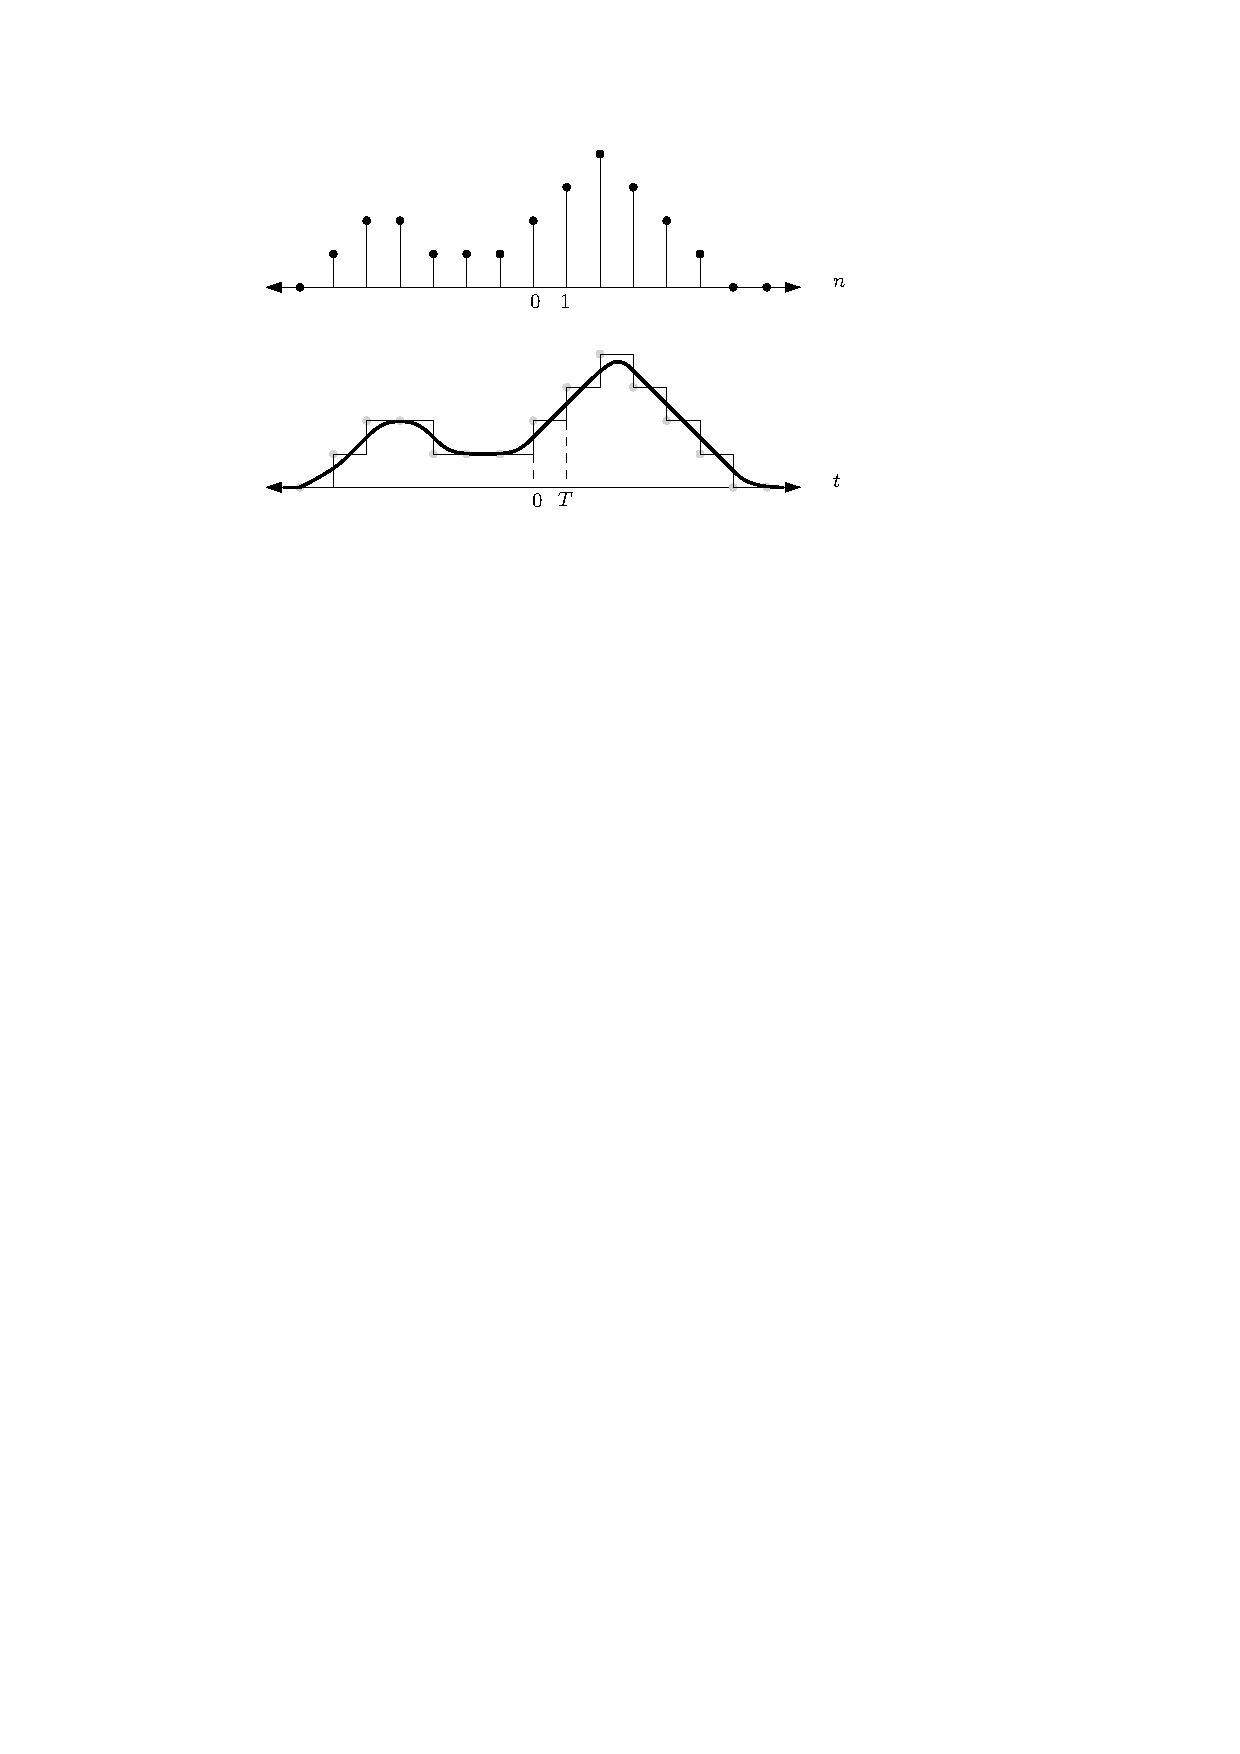
\includegraphics[scale=1]{graphics/sinc-interp.pdf}
\end{center}

In general the reconstruction filter is of a similar, or identical form to the anti-aliasing filter.
